\chapter{Scope}\label{scope}

The scope of modeling plant loops in EnergyPlus is limited depending on the application. For example, there is no provision to model nested loops, and multiple splitter-mixer pairs in a single loop which are often used in large scale systems. Thus, it has to be realized that modeling large scale district loops may be challenging in EnergyPlus. One way to model such systems is to make some assumptions to condense some arrangements of components that cannot be modeled in EnergyPlus. This approach may not work because the arrangements could be very important to the system. Figure~\ref{fig:central-plant-chilled-water-schematic-for} shows a central plant chilled water system for the University of California, Riverside (Hyman and Little, 2004). This system contains a total of eight splitter-mixer pairs, four on the supply side, and four on the demand side. We could make some assumptions to simplify the system. For example we can use a single chiller instead of the array of five chillers, this could work if we size and control the chiller properly, but the concept of scheduling the different chillers to operate at different times of the day to improve efficiency will be lost. Hence, it should be noted that while simplifications can provide a general overview of how the system will operate, they may defeat the original purpose of the complex design. Therefore, this guide will only discuss building plant systems which are less complicated.

\begin{figure}[hbtp] % fig 1
\centering
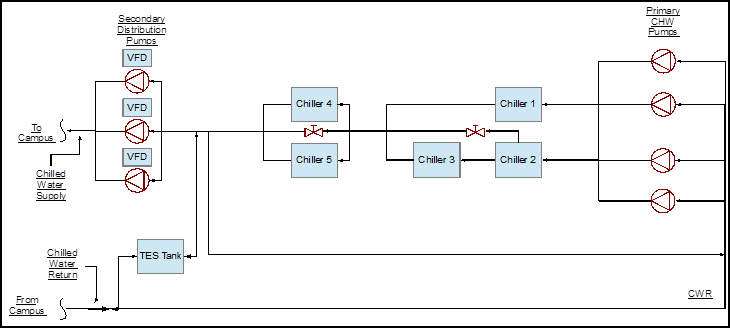
\includegraphics[width=0.9\textwidth, height=0.9\textheight, keepaspectratio=true]{media/image001.png}
\caption{Central plant chilled water schematic for the University of California, Riverside (recreated from Hyman and Little, 2004) \protect \label{fig:central-plant-chilled-water-schematic-for}}
\end{figure}
